\chapter{Benutzeroberfläche}
    Die Hauptaufgabe unserer \gls{GUI} liegt darin Workflow-Anwendungen zu erstellen. Die Erstellung und Einsicht von Workflow-Anwendungen ist erst nachdem Anmelden sichtbar. Es gibt folgende Ansichten:
    \begin{itemize}
        \item Login/Logout \ref{fig:Abb 1}
        \item Registrierung \ref{fig:Abb 2}
        \item Administration \ref{fig:Abb 3}
        \item Workflow Design \ref{fig:Abb 4}
        \item Workflow Ausführung \ref{fig:sfig3}
        \item Informationen zu Workflows \ref{fig:Abb 6}
    \end{itemize}

\begin{figure}[ht]
    \centering
    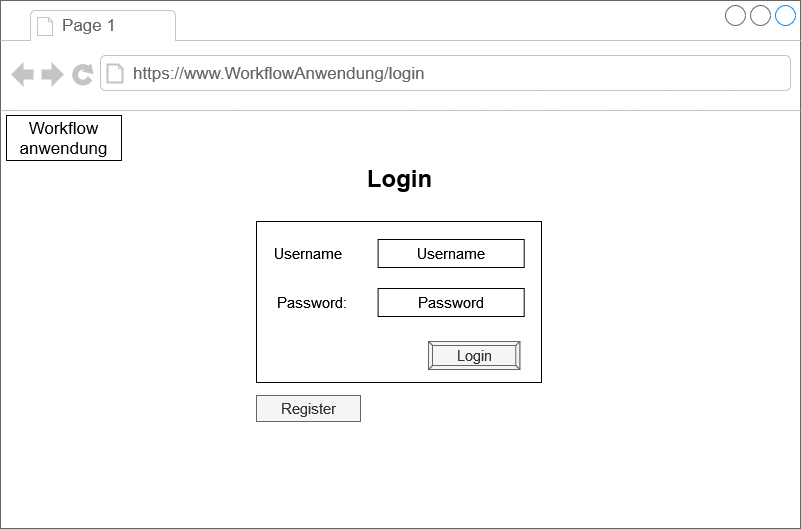
\includegraphics[width = 0.75\textwidth]{Grafiken/Gui Mockups/loginGui.drawio.png}
    \caption{Login Seite}
    \label{fig:Abb 1}
\end{figure}

\begin{figure}[ht]
    \centering
    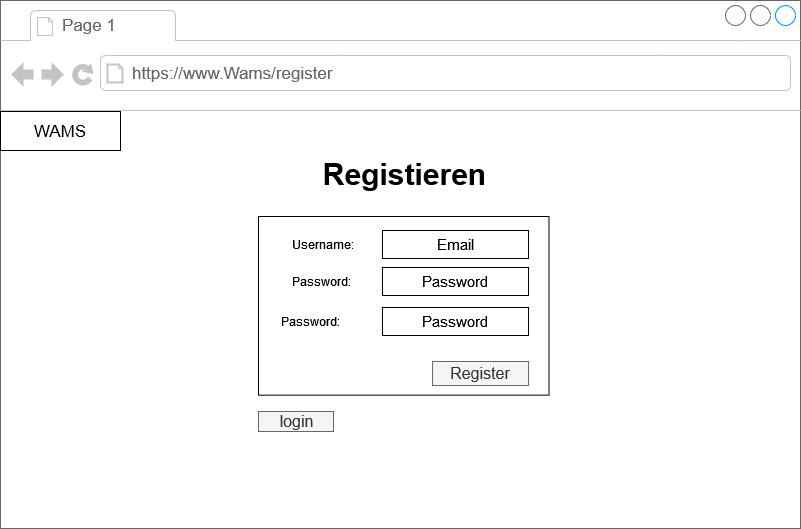
\includegraphics[width = 0.75\textwidth]{Grafiken/Gui Mockups/registrationGui.drawio.png}
    \caption{Registrierungsseite}
    \label{fig:Abb 2}
\end{figure}

\begin{figure}[ht]
    \centering
    \begin{subfigure}{.75\textwidth}
        \centering
        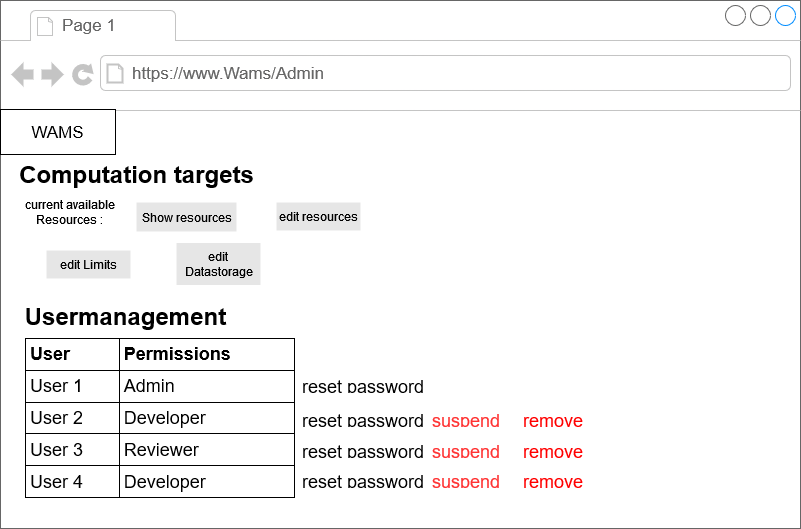
\includegraphics[width = \textwidth]{Grafiken/Gui Mockups/workflowGui-admin.drawio.png}
        \caption{Administration}
        \label{fig:sfig1}
    \end{subfigure}
   \begin{subfigure}{.75\textwidth}
    \centering
    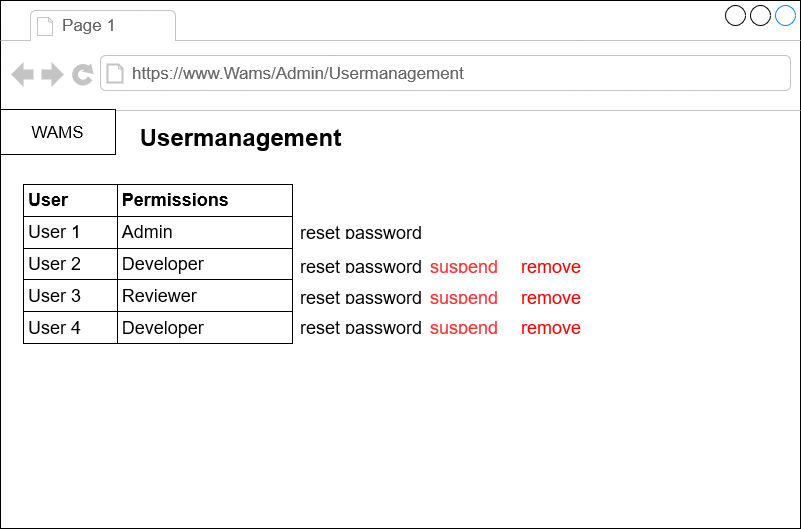
\includegraphics[width = \textwidth]{Grafiken/Gui Mockups/nutzerverwaltungGui.drawio.png}
    \caption{Nutzerverwaltung}
    \label{fig:sfig2}
   \end{subfigure}
   \caption{Administartionsseiten}
   \label{fig:Abb 3}
\end{figure}
    
\begin{figure}[ht]
    \centering
    \begin{subfigure}{.75\textwidth}
        \centering
        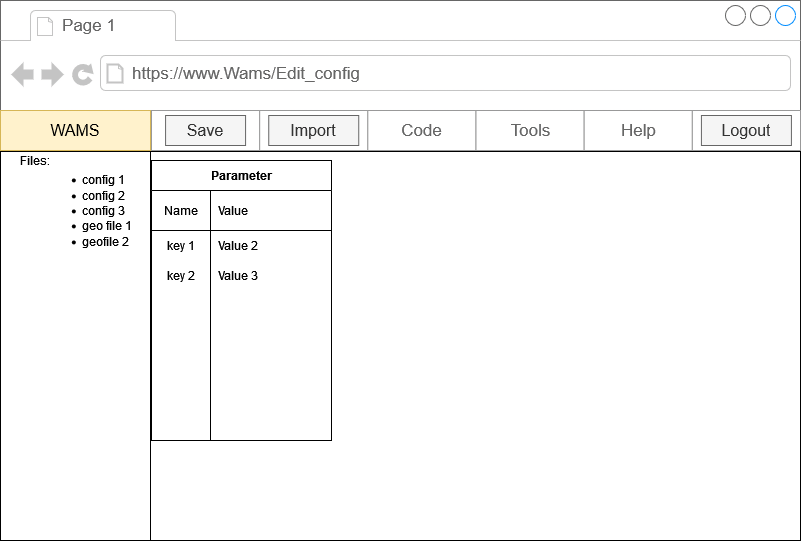
\includegraphics[width = \textwidth]{Grafiken/Gui Mockups/workflowGui-ConfigEdit.drawio.png}
    \caption{Bearbeiten von Konfig dateien}
    \label{fig: sfigKonfig}
    \end{subfigure}
   \begin{subfigure}{.75\textwidth}
    \centering
    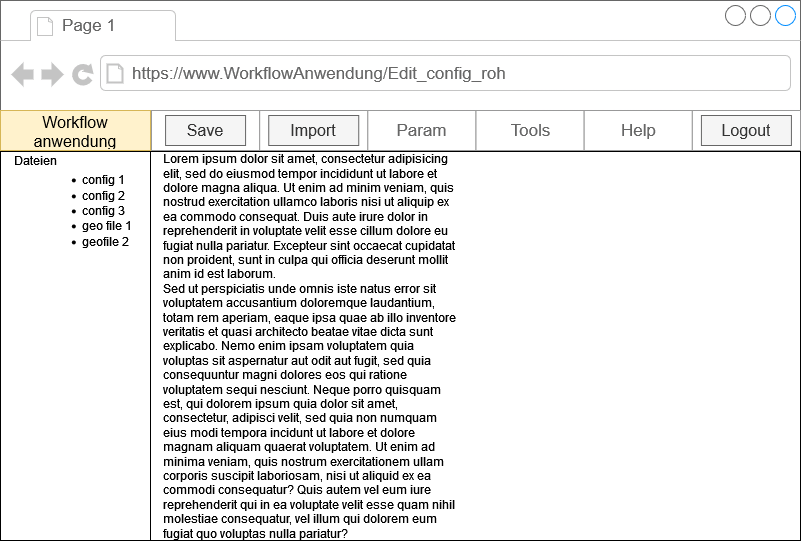
\includegraphics[width = \textwidth]{Grafiken/Gui Mockups/workflowGui-ConfigEditRohdata.drawio.png}
    \caption{Bearbeiten von Roh-Konfig Dateien}
    \label{fig:sfigRawConfig}
   \end{subfigure}
   \begin{subfigure}{.75\textwidth}
        \centering
        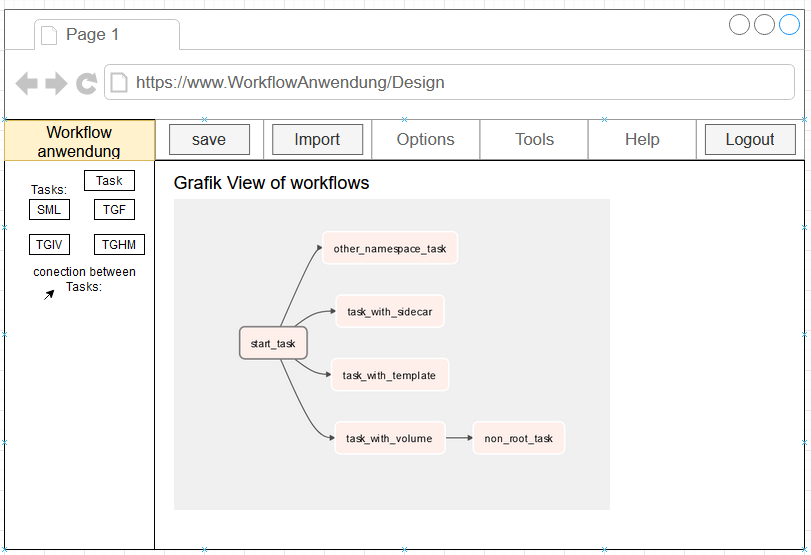
\includegraphics[width = \textwidth]{Grafiken/Gui Mockups/workflowGui-Design.drawio.png}
        \caption{Designen von Workflows mit Grafischer Oberfläche}
        \label{fig:sfigGraficDesign}
   \end{subfigure}
   \caption{Bearbeiten der Konfigdateien und Workflows}
   \label{fig:Abb 4}
\end{figure}
    

\begin{figure}[ht]
    \begin{subfigure}{.75\textwidth}
        \centering
        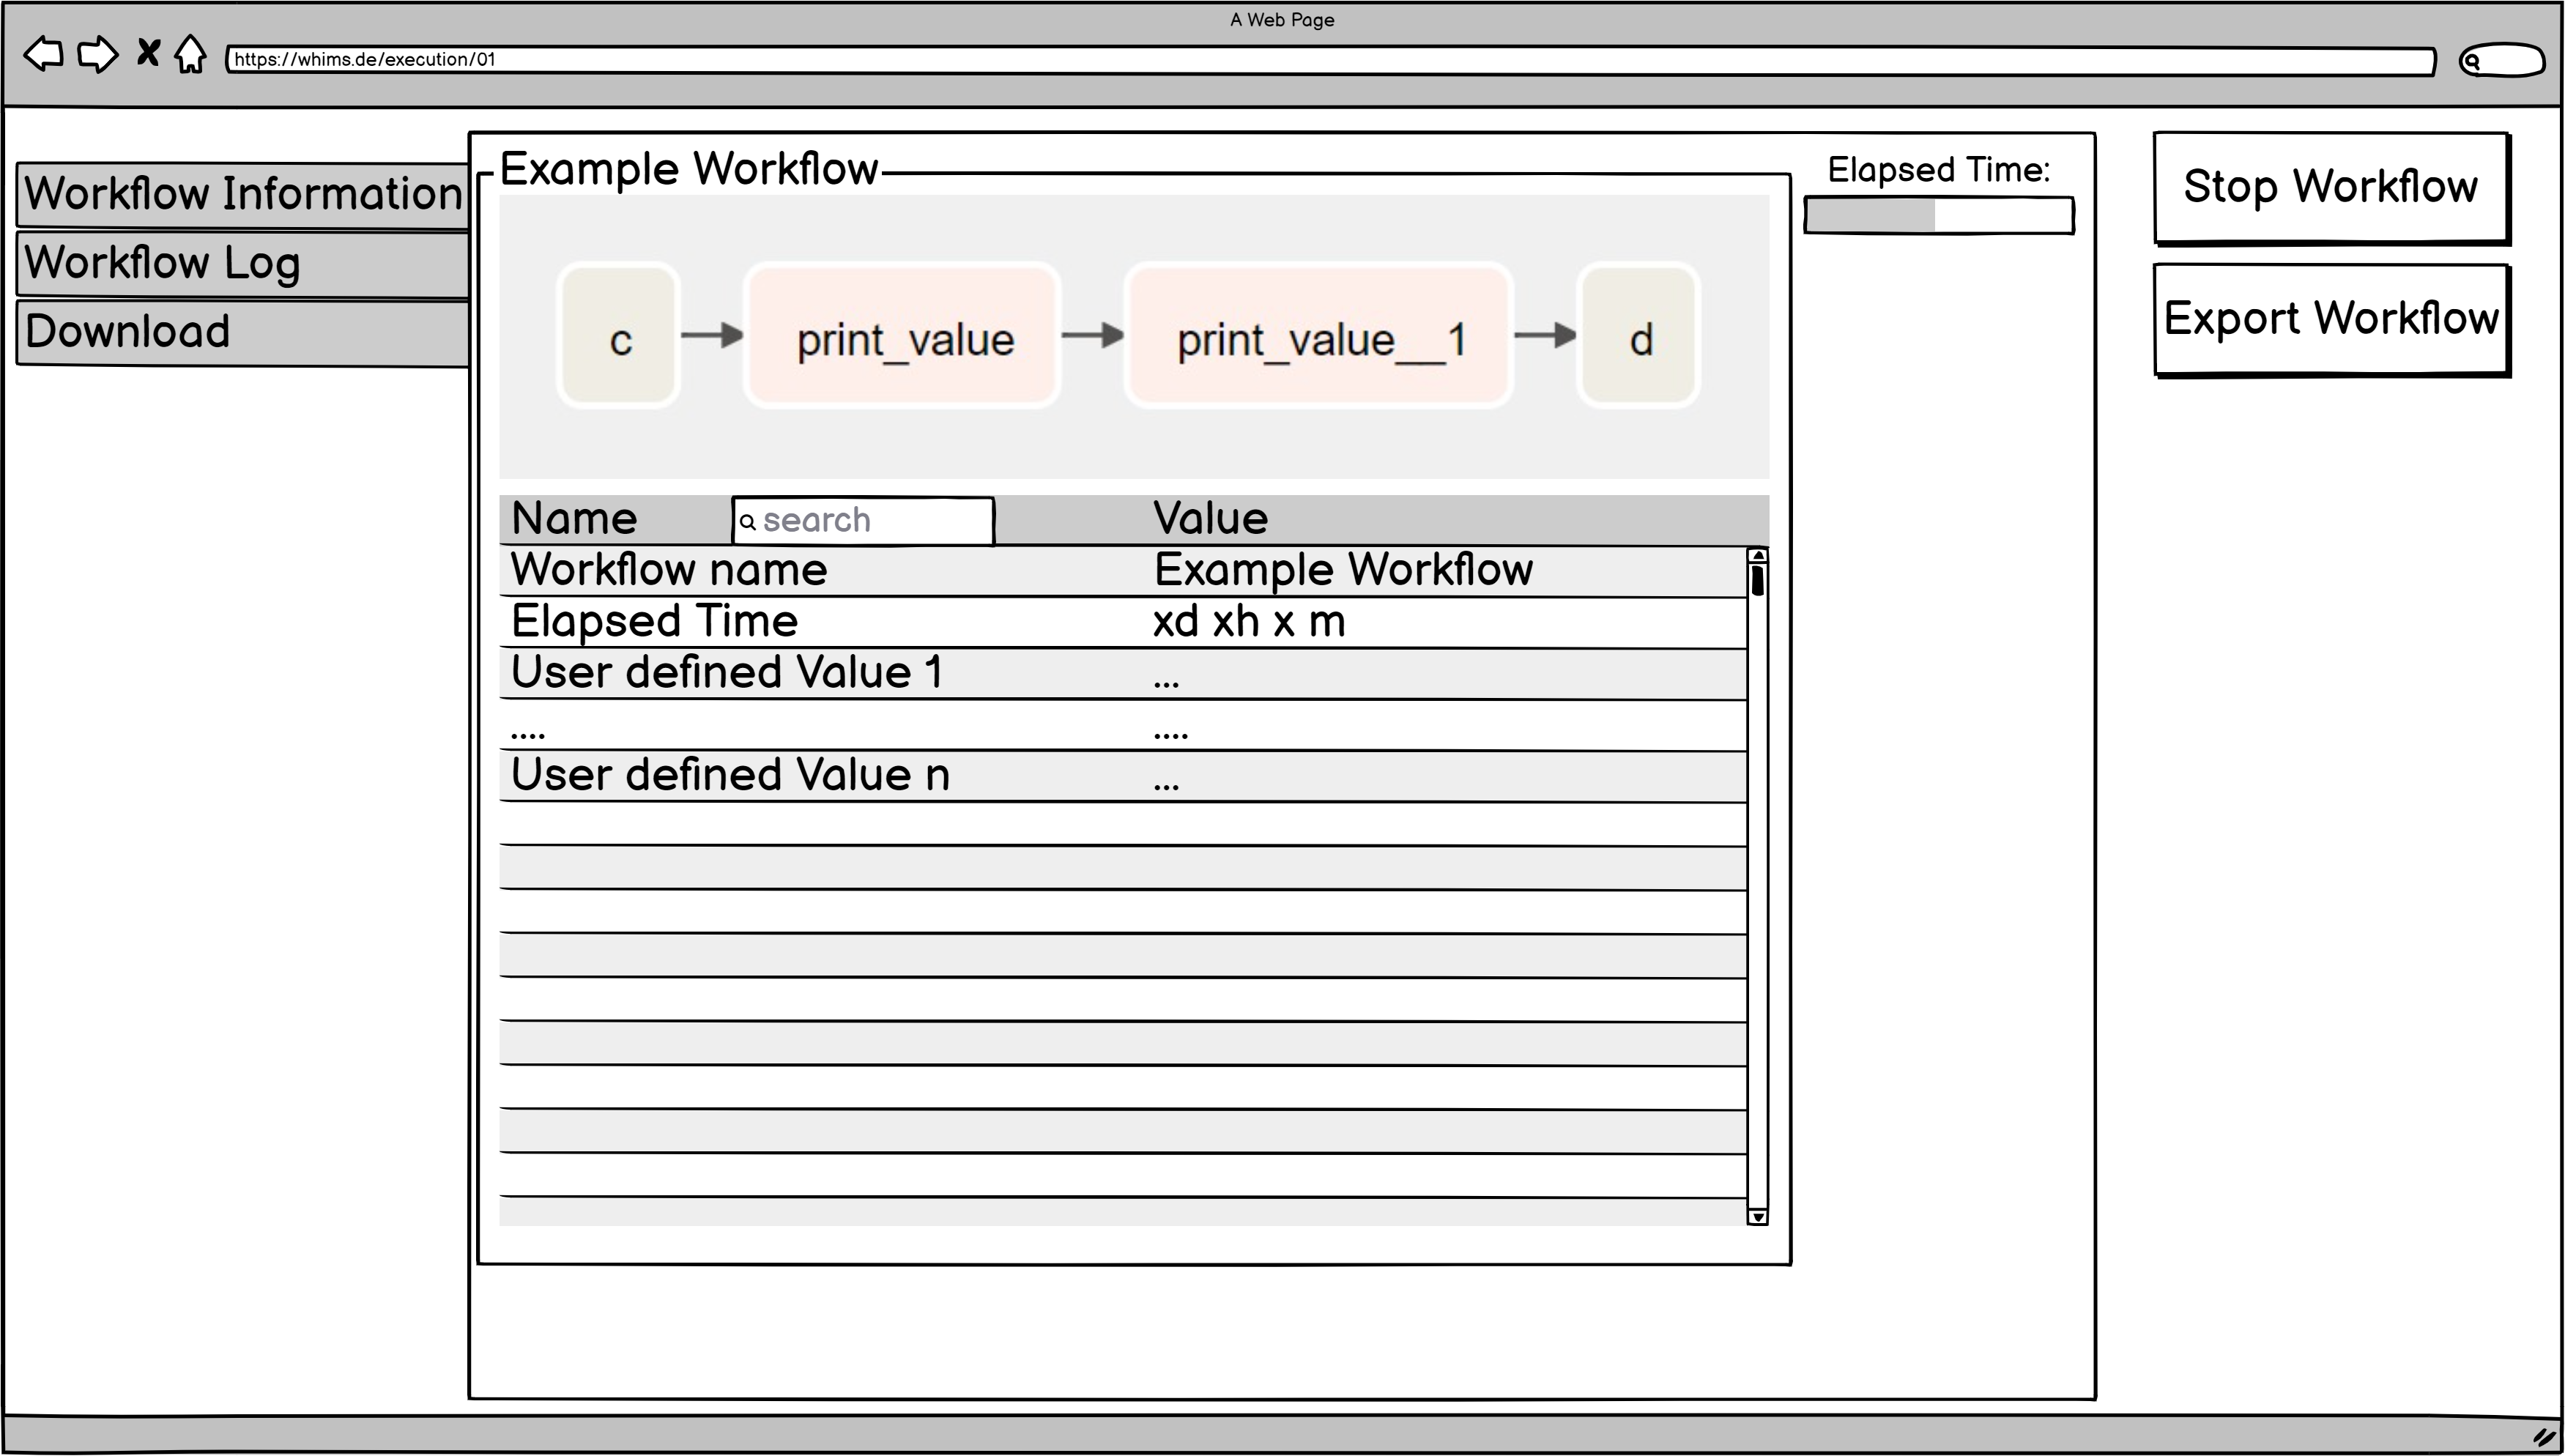
\includegraphics[width = \textwidth]{Grafiken/Gui Mockups/workflowGui-InformationMain.png}
        \caption{1 - Hauptseite}
        \label{fig:sfig3}
    \end{subfigure}
    \begin{subfigure}{.75\textwidth}
        \centering
        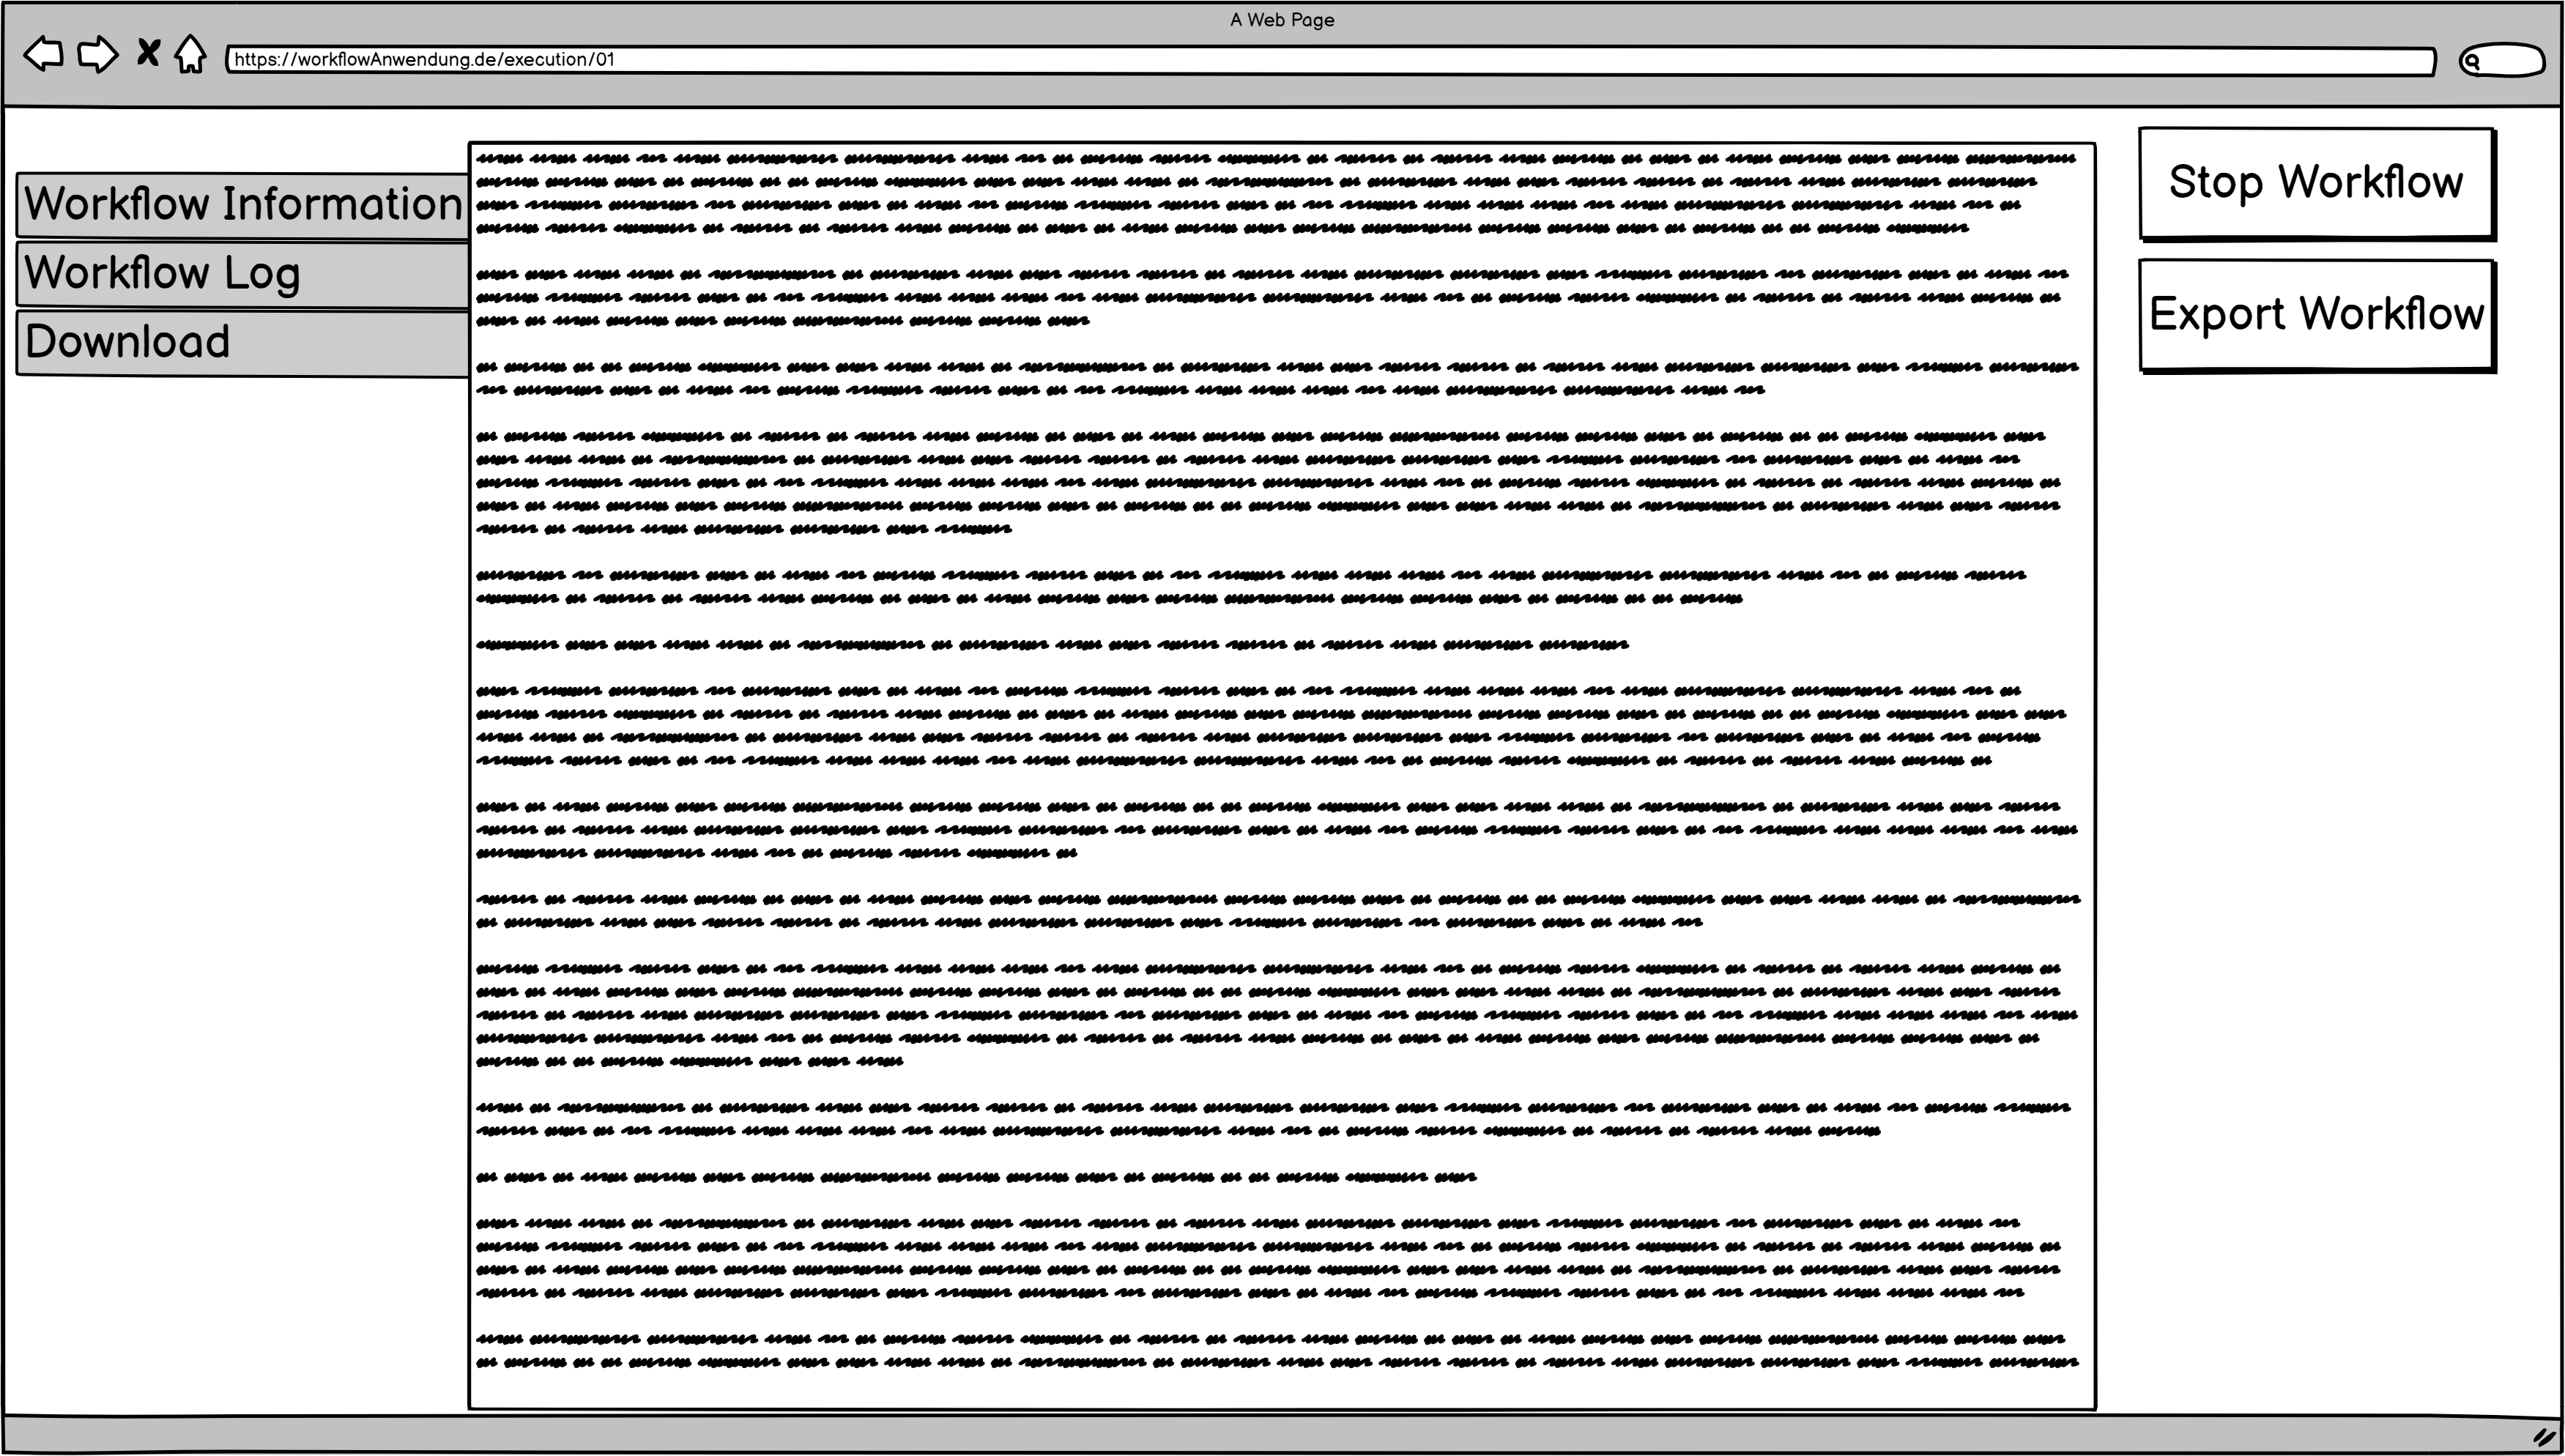
\includegraphics[width = \textwidth]{Grafiken/Gui Mockups/workflowGui-InformationLog.png}
        \caption{2 - Workflow Log}
        \label{fig:sfig4}
    \end{subfigure}
    \begin{subfigure}{.75\textwidth}
        \centering
        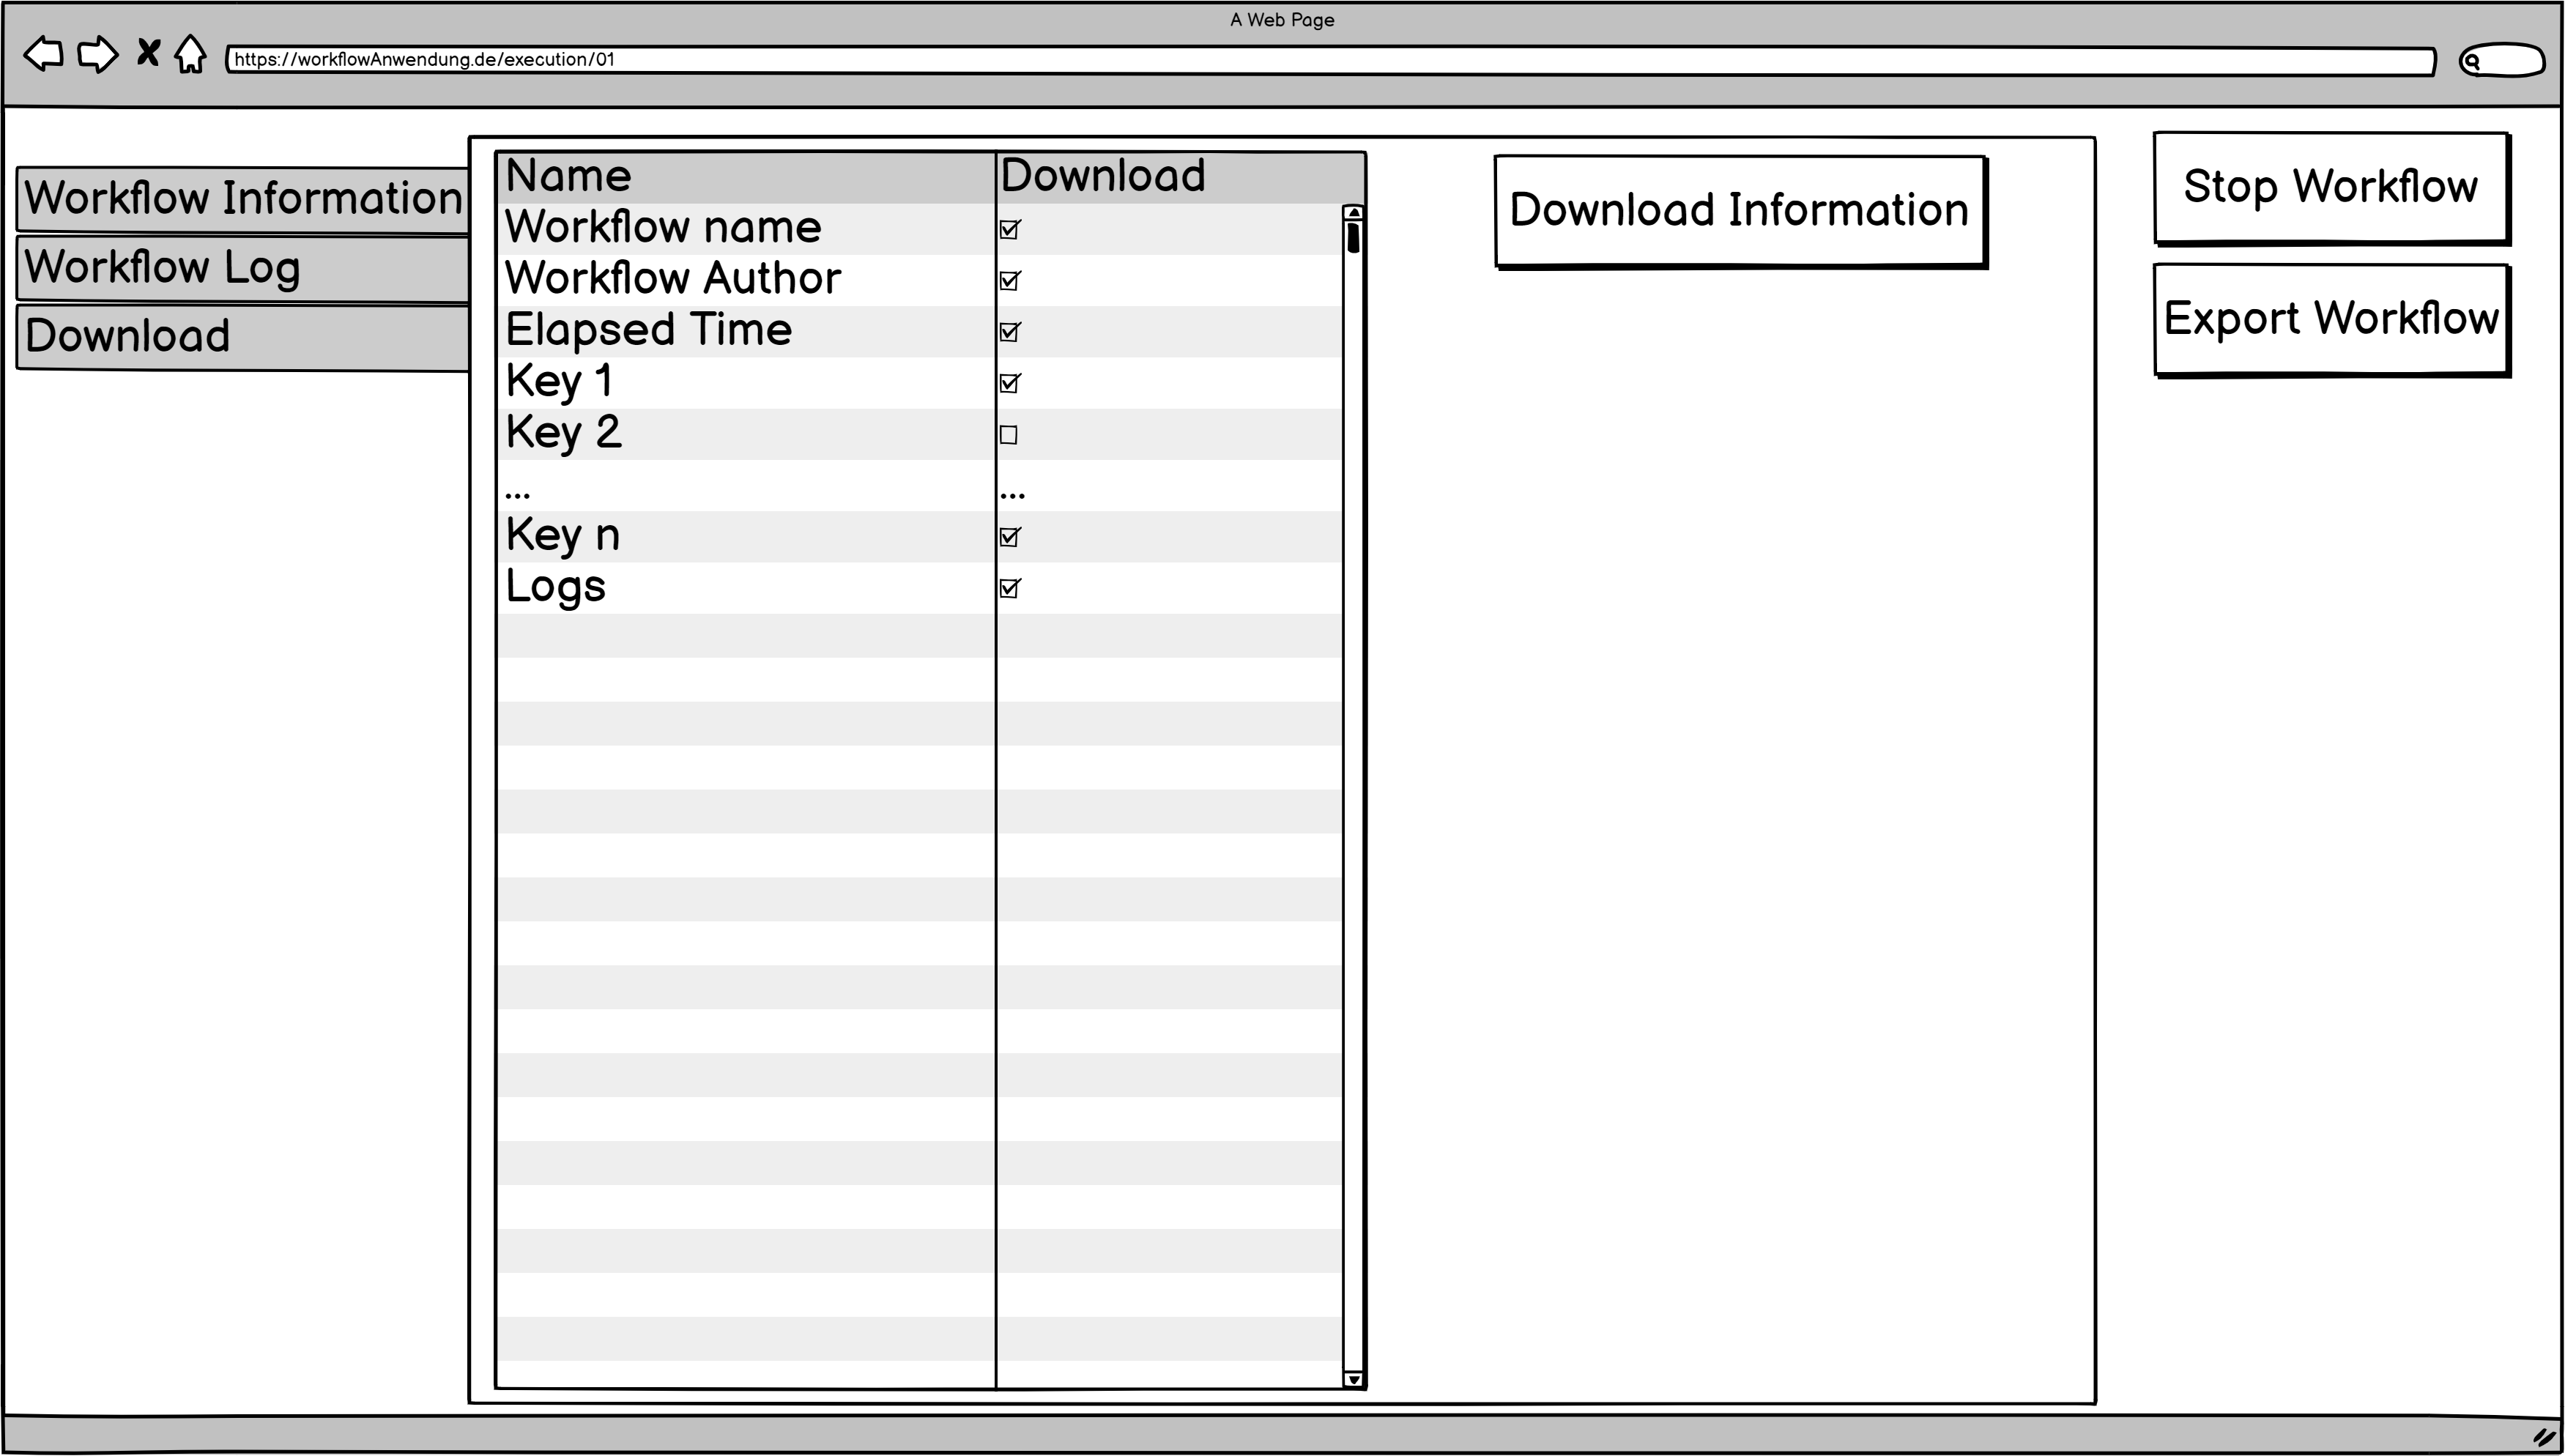
\includegraphics[width = \textwidth]{Grafiken/Gui Mockups/workflowGui-InformationDownload.png}
        \caption{3 - Informationen Herunterladen}
        \label{fig:sfig5}
    \end{subfigure}
    \centering
    \caption{Informationen zu Workflows}
    \label{fig:Abb 6}
\end{figure}
